\documentclass[11pt,fleqn]{article}

\usepackage[margin=1in]{geometry}
\usepackage{parskip}
\usepackage{enumitem}
\usepackage{amsmath}    % Better math support
\usepackage{amssymb}    % Optional: additional math symbols
\usepackage{tikz}       % fancy polynomial long division
\usetikzlibrary{calc}

\NewDocumentCommand{\EId}{}{%

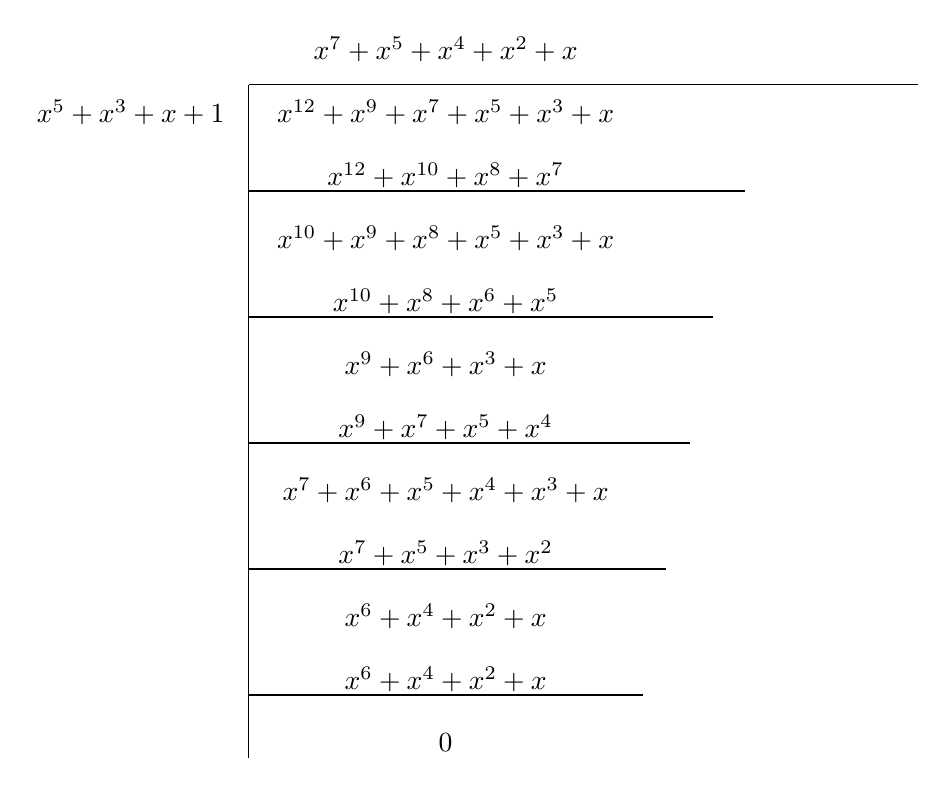
\begin{tikzpicture}[font=\normalsize]

% Coordinates are now the center of each node
% and all rows share the same x-coordinate

% Dividend
\node (A) at (2,0)
{$x^{12}+x^9+x^7+x^5+x^3+x$};

% Divisor
\node at (-2,0)
{$x^5+x^3+x+1$};

% Division symbol
\draw (-0.5,0.35)--(-0.5,-8.2);
\draw (-0.5,0.35)--(8,0.35);

% Quotient
\node at (2,0.8)
{$x^7+x^5+x^4+x^2+x$};

% Step 1
\node at (2,-0.8)
{$x^{12}+x^{10}+x^8+x^7$};

\draw (-.5,-1.0)--(5.8,-1.0);

\node at (2,-1.6)
{$x^{10}+x^9+x^8+x^5+x^3+x$};

% Step 2
\node at (2,-2.4)
{$x^{10}+x^8+x^6+x^5$};

\draw (-.5,-2.6)--(5.4,-2.6);

\node at (2,-3.2)
{$x^9+x^6+x^3+x$};

% Step 3
\node at (2,-4.0)
{$x^9+x^7+x^5+x^4$};

\draw (-.5,-4.2)--(5.1,-4.2);

\node at (2,-4.8)
{$x^7+x^6+x^5+x^4+x^3+x$};

% Step 4
\node at (2,-5.6)
{$x^7+x^5+x^3+x^2$};

\draw (-.5,-5.8)--(4.8,-5.8);

\node at (2,-6.4)
{$x^6+x^4+x^2+x$};

% Step 5
\node at (2,-7.2)
{$x^6+x^4+x^2+x$};

\draw (-.5,-7.4)--(4.5,-7.4);

\node at (2,-8.0)
{$0$};

\end{tikzpicture}
}

\NewDocumentCommand{\EIIa}{}{%
\begin{tikzpicture}[font=\small]
% Dividend
\node (A) at (2,0)
{$x^6+x^5+x^3+x^2+1$};

% Divisor
\node at (-2,0)
{$x^3+x+1$};

% Division bracket
\draw (-0.5,0.35)--(-0.5,-6.8);
\draw (-0.5,0.35)--(7,0.35);

% Quotient
\node at (2,0.8)
{$x^3+x^2+x+1$};

% Step 1
\node at (2,-0.8)
{$x^6+x^4+x^3$};

\draw (-.5,-1.0)--(4.8,-1.0);

\node at (2,-1.6)
{$x^5+x^4+x^2+1$};


% Step 2
\node at (2,-2.4)
{$x^5+x^3+x^2$};

\draw (-.5,-2.6)--(4.5,-2.6);

\node at (2,-3.2)
{$x^4+x^3+1$};


% Step 3
\node at (2,-4.0)
{$x^4+x^2+x$};

\draw (-.5,-4.2)--(4.3,-4.2);

\node at (2,-4.8)
{$x^3+x^2+x+1$};


% Step 4
\node at (2,-5.6)
{$x^3+x+1$};

\draw (-.5,-5.8)--(4.0,-5.8);

\node at (2,-6.4)
{$x^2$};
\end{tikzpicture}

}

\NewDocumentCommand{\EIIIb}{}{%
\begin{tikzpicture}[font=\small]

% Dividend
\node (A) at (2,0)
{$x^4+x^3+1$};

% Divisor
\node at (-2,0)
{$x^2+x+1$};

% Division bracket
\draw (-0.5,0.35)--(-0.5,-4);
\draw (-0.5,0.35)--(5.5,0.35);

% Quotient
\node at (2,0.8)
{$x^2+1$};

%--------------------------------------------------
% Step 1
%--------------------------------------------------
\node at (2,-0.8)
{$x^4+x^3+x^2$};

\draw (-.5,-1.0)--(4.3,-1.0);

\node at (2,-1.6)
{$x^2+1$};

%--------------------------------------------------
% Step 2
%--------------------------------------------------
\node at (2,-2.4)
{$x^2+x+1$};

\draw (-.5,-2.6)--(3.8,-2.6);

\node at (2,-3.2)
{$x$};

\end{tikzpicture}

}

\NewDocumentCommand{\EVa}{}{%
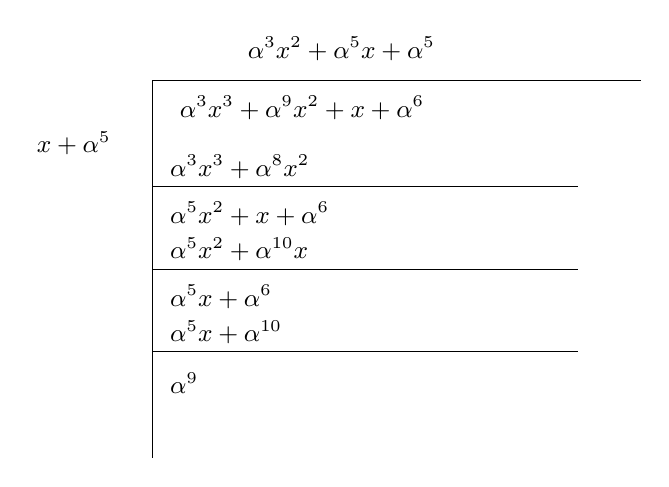
\begin{tikzpicture}[font=\small]

% Quotient
\node at (4.2,1.2)
{$\alpha^3x^2+\alpha^5x+\alpha^5$};

% Main division bracket
\draw (1.8,0.8) -- (1.8,-4.0);
\draw (1.8,0.8) -- (8.0,0.8);

% Divisor
\node at (0.8,0.0)
{$x+\alpha^5$};

% Dividend
\node at (3.7,0.45)
{$\alpha^3x^3+\alpha^9x^2+x+\alpha^6$};


% First addition step
\node[anchor=west] at (1.9,-0.3)
{$\alpha^3x^3+\alpha^8x^2$};

\draw (1.8,-0.55) -- (7.2,-0.55);

\node[anchor=west] at (1.9,-0.9)
{$\alpha^5x^2+x+\alpha^6$};


% Second addition step
\node[anchor=west] at (1.9,-1.35)
{$\alpha^5x^2+\alpha^{10}x$};

\draw (1.8,-1.6) -- (7.2,-1.6);

\node[anchor=west] at (1.9,-1.95)
{$\alpha^5x+\alpha^6$};


% Third addition step
\node[anchor=west] at (1.9,-2.4)
{$\alpha^5x+\alpha^{10}$};

\draw (1.8,-2.65) -- (7.2,-2.65);

% Remainder
\node[anchor=west] at (1.9,-3.05)
{$\alpha^9$};

\end{tikzpicture}
}

\begin{document}

%==================================================
% Title
%==================================================

\begin{flushleft}
    {\LARGE \textbf{Álgebra en FEC (II)}}\\[0.5em]
    {\large Ferraris Domingo}\\[0.5em]
    \today
\end{flushleft}

\vspace{0.5em}
\hrule
\vspace{1em}

%==================================================
% Summary
%==================================================

\section*{Resumen}

\subsection*{Ejercicio 1 Polinomios sobre GF(2)}
\begin{enumerate}[label=\alph*)]
\item \boxed{
    \begin{aligned}
        a&=0b1101010=1+x+x^3+x^5\\
        b&=0b01101101=x+x^2+x^4+x^5+x^7
    \end{aligned}
}
\item \boxed{a+b=1+x^2+x^3+x^4+x^7=0b10111001}
\item \boxed{a\cdot b=x+x^3+x^5+x^7+x^9+x^{12}=0b0101010101001}
\item \boxed{\frac{a\cdot b}{a}=x^7+x^5+x^4+x^2+x=b}
\end{enumerate}

\subsection*{Ejercicio 2 División de polinomios}
\begin{enumerate}[label=\alph*)]
\item \boxed{\frac{f}{g}=\frac{x^6+x^5+x^3+x^2+1}{x^3+x+1}\iff q=x^3+x^2+x+1,\quad r=x^2}
\item \boxed{f=x^6+x^5+x^3+x^2+1=q\cdot g+r=(x^3+x^2+x+1)\cdot (x^3+x+1)+x^2}
\end{enumerate}

\subsection*{Ejercicio 3 Polinomios irreducibles y primitivos}
\begin{enumerate}[label=\alph*)]
\item \boxed{p=x^4+x^3+1 \implies Raices\notin GF(2)}
\item \boxed{\frac{x^4+x^3+1}{x^2+x+1}\implies r=x\neq0 \therefore\text{Irreducible sobre GF(2)}}
\item \boxed{
\large
\begin{array}{l|l|l}
    \hline
\text{Potencia}& \text{Polinomica}             & \text{Tupla} \\
\hline
0           & 0                             & 0b0000    \\
1           & 1                             & 0b1000    \\
\alpha^1    & \alpha                        & 0b0100    \\
\alpha^2    & \alpha^2                      & 0b0010    \\
\alpha^3    & \alpha^3                      & 0b0001    \\
\alpha^4    & \alpha^3+1                    & 0b1001    \\
\alpha^5    & \alpha^3+\alpha+1             & 0b1101    \\
\alpha^6    & \alpha^3+\alpha^2+\alpha+1    & 0b1111    \\
\alpha^7    & \alpha^2+\alpha+1             & 0b1110    \\
\alpha^8    & \alpha^3+\alpha^2+\alpha      & 0b0111    \\
\alpha^9    & \alpha^2+1                    & 0b1010    \\
\alpha^{10} & \alpha^3+\alpha               & 0b0101    \\
\alpha^{11} & \alpha^3+\alpha^2+1           & 0b1011    \\
\alpha^{12} & \alpha+1                      & 0b1100    \\
\alpha^{13} & \alpha^2+\alpha               & 0b0110    \\
\alpha^{14} & \alpha^3+\alpha^2             & 0b0011    \\
\hline
\end{array}
}
\end{enumerate}

\subsection*{Ejercicio 4 Suma y producto de polinomios sobre $GF(2^4)$}
\begin{enumerate}[label=\alph*)]
\item \boxed{f+g=(\alpha^3x^2+\alpha^7x+\alpha^2)+(\alpha^5x+\alpha^{10})=\alpha^3x^2+\alpha^{14}x+\alpha^8}
\item \boxed{f\cdot g=(\alpha^3x^2+\alpha^7x+\alpha^2)\cdot(\alpha^5x+\alpha^{10})=\alpha^8x^3+\alpha^9x^2+\alpha^{12}x+\alpha^{12}}
\end{enumerate}

\subsection*{Ejercicio 5 División y potencia de polinomios sobre $GF(2^4)$}
\begin{enumerate}[label=\alph*)]
\item \boxed{\frac{f}{g}=\frac{\alpha^3x^3+\alpha^9x^2+x+\alpha^6}{x+\alpha^5}\iff q=\alpha^3x^2+\alpha^5x+\alpha^5,\quad r=\alpha^9}
\item \boxed{h^2=(\alpha^3x^2+\alpha^{11}x+\alpha^6)^2=\alpha^6x^4+\alpha^7x^2+\alpha^{12}}
\end{enumerate}

\subsection*{Ejercicio 6 Búsqueda de raíces}
\begin{enumerate}[label=\alph*)]
\item \boxed{f=x^2+\alpha^5x+\alpha^9=(x+\alpha^{11})\cdot(x+\alpha^{13})}
\end{enumerate}

\subsection*{Ejercicio 7 Ortogonalidad sobre GF(2)}
\begin{enumerate}[label=\alph*)]
\item \boxed{u\cdot v=(1,1,0,1)\cdot(0,1,1,1)=0\implies \text{u ortogonal a v en GF(2)}}
\item \boxed{w=(1,1)\in V_2 \text{ w ortogonal a si mismo sobre GF(2)}}
\end{enumerate}

\subsection*{Ejercicio 8 Matriz generadora, forma sistemática y matriz de verificación}
\begin{enumerate}[label=\alph*)]
\item \boxed{
G=\begin{bmatrix}
1&1&0&0&1&1\\
0&1&1&1&0&1\\
0&0&1&0&1&1
\end{bmatrix}
\implies G_{sis}=[I_3\mid P]=
\begin{bmatrix}
1&0&0&1&0&1\\
0&1&0&1&1&0\\
0&0&1&0&1&1
\end{bmatrix}
}
\item \boxed{
H=[P^T\mid I_3]=
\begin{bmatrix}
1&1&0&1&0&0\\
0&1&1&0&1&0\\
1&0&1&0&0&1
\end{bmatrix}
}
\item \boxed{G_{sis}H^T=[0]}
\item \boxed{u=(1,0,1)\rightarrow v=(1,0,1,1,1,0)}
\item \boxed{\text{Codeword de la suma igual a la suma de codewords}}
\end{enumerate}

\vspace{1em}
\hrule
\vspace{1em}

%==================================================
% Details
%==================================================

\section*{Desarrollo}

\subsection*{Ejercicio 1 Polinomios sobre GF(2)}
\begin{enumerate}[label=\alph*)]
\item \boxed{
    \begin{aligned}
        a&=0b1101010=1+x+x^3+x^5\\
        b&=0b01101101=x+x^2+x^4+x^5+x^7
    \end{aligned}
}

\item \boxed{a+b=1+x^2+x^3+x^4+x^7=0b10111001}
\begin{align*}
    a+b
    &=(1+x+x^3+x^5)+(x+x^2+x^4+x^5+x^7)\\
    &=1+x+x^3+x^5+x+x^2+x^4+x^5+x^7\\
    &=1+(x+x)+x^2+x^3+x^4+(x^5+x^5)+x^7\\
    &=1+x^2+x^3+x^4+x^7\\
    &=0b10111001
\end{align*}

\item \boxed{a\cdot b=x+x^3+x^5+x^7+x^9+x^{12}=0b0101010101001}
\begin{align*}
a\cdot b
&=(1+x+x^3+x^5)\cdot(x+x^2+x^4+x^5+x^7)\\
&=1\cdot(x+x^2+x^4+x^5+x^7)+x\cdot(x+x^2+x^4+x^5+x^7)\\
&+x^3\cdot(x+x^2+x^4+x^5+x^7)+x^5\cdot(x+x^2+x^4+x^5+x^7)\\ \\
&=(x+x^2+x^4+x^5+x^7)+(x^2+x^3+x^5+x^6+x^8)\\
&+(x^4+x^5+x^7+x^8+x^{10})+(x^6+x^7+x^9+x^{10}+x^{12})\\ \\
&=x+0+x^3+0+x^5+0+x^7+0+x^9+0+x^{12}\\
&=x+x^3+x^5+x^7+x^9+x^{12}\\
&=0b0101010101001
\end{align*}

\item \boxed{\frac{a\cdot b}{a}=x^7+x^5+x^4+x^2+x=b}
\\ \\
\EId
\end{enumerate}

\subsection*{Ejercicio 2 División de polinomios}
\begin{enumerate}[label=\alph*)]
\item \boxed{\frac{f}{g}=\frac{x^6+x^5+x^3+x^2+1}{x^3+x+1}\iff q=x^3+x^2+x+1,\quad r=x^2}

\EIIa

\item \boxed{f=x^6+x^5+x^3+x^2+1=q\cdot g+r=(x^3+x^2+x+1)\cdot (x^3+x+1)+x^2}
\begin{align*}
    x^6+x^5+x^3+x^2+1
    &\overset{?}{=}(x^3+x^2+x+1)\cdot (x^3+x+1)+x^2\\
    &\overset{?}{=}x^3\cdot (x^3+x+1)+x^2\cdot (x^3+x+1)\\
    &+x\cdot (x^3+x+1)+1\cdot (x^3+x+1)+x^2\\
    &=x^6+x^5+x^3+x^2+1
\end{align*}

\end{enumerate}

\subsection*{Ejercicio 3 Polinomios irreducibles y primitivos}
\begin{enumerate}[label=\alph*)]
\item \boxed{p=x^4+x^3+1 \implies Raices\notin GF(2)}
\begin{align*}
p(0)
&=0^4+0^3+1=1\neq 0\\
p(1)
&=1^4+1^3+1=1\neq0
\end{align*}

\item \boxed{\frac{x^4+x^3+1}{x^2+x+1}\implies r=x\neq0 \therefore\text{Irreducible sobre GF(2)}}

\EIIIb

\item \boxed{
\large
\begin{array}{l|l|l}
    \hline
\text{Potencia}& \text{Polinomica}             & \text{Tupla} \\
\hline
0           & 0                             & 0b0000    \\
1           & 1                             & 0b1000    \\
\alpha^1    & \alpha                        & 0b0100    \\
\alpha^2    & \alpha^2                      & 0b0010    \\
\alpha^3    & \alpha^3                      & 0b0001    \\
\alpha^4    & \alpha^3+1                    & 0b1001    \\
\alpha^5    & \alpha^3+\alpha+1             & 0b1101    \\
\alpha^6    & \alpha^3+\alpha^2+\alpha+1    & 0b1111    \\
\alpha^7    & \alpha^2+\alpha+1             & 0b1110    \\
\alpha^8    & \alpha^3+\alpha^2+\alpha      & 0b0111    \\
\alpha^9    & \alpha^2+1                    & 0b1010    \\
\alpha^{10} & \alpha^3+\alpha               & 0b0101    \\
\alpha^{11} & \alpha^3+\alpha^2+1           & 0b1011    \\
\alpha^{12} & \alpha+1                      & 0b1100    \\
\alpha^{13} & \alpha^2+\alpha               & 0b0110    \\
\alpha^{14} & \alpha^3+\alpha^2             & 0b0011    \\
\hline
\end{array}
}

\begin{align*}
\alpha^4+\alpha^3+1&=0\implies\alpha^4=\alpha^3+1\\
\alpha^0 &= 1\\
\alpha^1 &= \alpha\\
\alpha^2 &= \alpha^2\\
\alpha^3 &= \alpha^3\\
\alpha^4 &= \alpha^3+1\\
\alpha^5 &= \alpha\alpha^4=\alpha(\alpha^3+1)=\alpha^4+\alpha=(\alpha^3+1)+\alpha=\alpha^3+\alpha+1\\
\alpha^6 &= \alpha(\alpha^3+\alpha+1)=\alpha^4+\alpha^2+\alpha=(\alpha^3+1)+\alpha^2+\alpha=\alpha^3+\alpha^2+\alpha+1\\
\alpha^7 &= \alpha(\alpha^3+\alpha^2+\alpha+1)=\alpha^4+\alpha^3+\alpha^2+\alpha=(\alpha^3+1)+\alpha^3+\alpha^2+\alpha=\alpha^2+\alpha+1\\
\alpha^8 &= \alpha(\alpha^2+\alpha+1)=\alpha^3+\alpha^2+\alpha\\
\alpha^9 &= \alpha(\alpha^3+\alpha^2+\alpha)= \alpha^4+\alpha^3+\alpha^2= (\alpha^3+1)+\alpha^3+\alpha^2= \alpha^2+1\\
\alpha^{10} &= \alpha(\alpha^2+1)= \alpha^3+\alpha\\
\alpha^{11} &= \alpha(\alpha^3+\alpha)= \alpha^4+\alpha^2= (\alpha^3+1)+\alpha^2= \alpha^3+\alpha^2+1\\
\alpha^{12} &= \alpha(\alpha^3+\alpha^2+1)= \alpha^4+\alpha^3+\alpha= (\alpha^3+1)+\alpha^3+\alpha= \alpha+1\\
\alpha^{13} &= \alpha(\alpha+1)= \alpha^2+\alpha\\
\alpha^{14} &= \alpha(\alpha^2+\alpha)= \alpha^3+\alpha^2\\
\alpha^{15} &= \alpha(\alpha^3+\alpha^2)= \alpha^4+\alpha^3= (\alpha^3+1)+\alpha^3= 1
\end{align*}

\end{enumerate}

\subsection*{Ejercicio 4 Suma y producto de polinomios sobre $GF(2^4)$}
\begin{enumerate}[label=\alph*)]
\item \boxed{f+g=(\alpha^3x^2+\alpha^7x+\alpha^2)+(\alpha^5x+\alpha^{10})=\alpha^3x^2+\alpha^{14}x+\alpha^8}
\begin{align*}
f+g
&=(\alpha^3x^2+\alpha^7x+\alpha^2)+(\alpha^5x+\alpha^{10})\\
&=\alpha^3x^2+(\alpha^7+\alpha^5)x+(\alpha^2+\alpha^{10})\\
&=\alpha^3x^2+\bigl((\alpha^2+\alpha+1)+(\alpha^3+\alpha+1)\bigr)x+\bigl(\alpha^2+(\alpha^3+\alpha)\bigr)\\
&=\alpha^3x^2+(\alpha^3+\alpha^2)x+(\alpha^3+\alpha^2+\alpha)\\
&=\alpha^3x^2+\alpha^{14}x+\alpha^8
\end{align*}

\item \boxed{f\cdot g=(\alpha^3x^2+\alpha^7x+\alpha^2)\cdot(\alpha^5x+\alpha^{10})=\alpha^8x^3+\alpha^9x^2+\alpha^{12}x+\alpha^{12}}
\begin{align*}
f\cdot g
&=(a^3x^2+a^7x+\alpha^2)\cdot(\alpha^5x+\alpha^{10})\\
&=\alpha^8x^3+\alpha^{13}x^2+\alpha^{12}x^2+\alpha^{17}x+\alpha^7x+\alpha^{12}\\
&=\alpha^8x^3+(\alpha^{13}+\alpha^{12})x^2+(\alpha^{17}+\alpha^7)x+\alpha^{12}\\
&=\alpha^8x^3+(\alpha^{13}+\alpha^{12})x^2+(\alpha^{2}+\alpha^7)x+\alpha^{12}\\
&=\alpha^8x^3+(\alpha^2+1)x^2+(\alpha^2+\alpha^2+\alpha+1)x+\alpha^{12}\\
&=\alpha^8x^3+\alpha^9x^2+\alpha^{12}x+\alpha^{12}
\end{align*}

\end{enumerate}

\subsection*{Ejercicio 5 División y potencia de polinomios sobre $GF(2^4)$}
\begin{enumerate}[label=\alph*)]
\item \boxed{\frac{f}{g}=\frac{\alpha^3x^3+\alpha^9x^2+x+\alpha^6}{x+\alpha^5}\iff q=\alpha^3x^2+\alpha^5x+\alpha^5,\quad r=\alpha^9}

\EVa


\item \boxed{h^2=(\alpha^3x^2+\alpha^{11}x+\alpha^6)^2=\alpha^6x^4+\alpha^7x^2+\alpha^{12}}
\begin{align*}
h^2
&=(\alpha^3x^2+\alpha^{11}x+\alpha^6)\cdot(\alpha^3x^2+\alpha^{11}x+\alpha^6)\\
&=\alpha^3x^2(\alpha^3x^2+\alpha^{11}x+\alpha^6)+\alpha^{11}x(\alpha^3x^2+\alpha^{11}x+\alpha^6)+\alpha^6(\alpha^3x^2+\alpha^{11}x+\alpha^6)\\
&=\alpha^6x^4+\alpha^{14}x^3+\alpha^9x^2+\alpha^{14}x^3+\alpha^{22}x^2+\alpha^{17}x+\alpha^9x^2+\alpha^{17}x+\alpha^{12}\\
&=\alpha^6x^4+(\alpha^{14}+\alpha^{14})x^3+(\alpha^9+\alpha^{22}+\alpha^9)x^2+(\alpha^{17}+\alpha^{17})x+\alpha^{12}\\
&=\alpha^6x^4+\alpha^{22}x^2+\alpha^{12}\\
&=\alpha^6x^4+\alpha^7x^2+\alpha^{12}
\end{align*}

\item Verificar el resultado anterior: elevar al cuadrado cada coeficiente de h(X) por separado y ubicarlo en el doble del grado correspondiente (identidad $(f(X))^2 = f(X^2)$)
\begin{align*}
h^2
&=(\alpha^3x^2+\alpha^{11}x+\alpha^6)^2\\
&=(\alpha^3x^2)^2+(\alpha^{11}x)^2+(\alpha^6)^2\\
&=\alpha^6x^4+\alpha^{22}x^2+\alpha^{12}\\
&=\alpha^6x^4+\alpha^{7}x^2+\alpha^{12}
\end{align*}

\end{enumerate}

\subsection*{Ejercicio 6 Búsqueda de raíces}
\begin{enumerate}[label=\alph*)]
\item \boxed{f=x^2+\alpha^5x+\alpha^9=(x+\alpha^{11})\cdot(x+\alpha^{13})}
\begin{align*}
f(\alpha^{11})
&=(\alpha^{11})^2+\alpha^5(\alpha^{11})+\alpha^9\\
&=\alpha^{22}+\alpha^{16}+\alpha^9\\
&=\alpha^7+\alpha+\alpha^9\\
&=(\alpha^2+\alpha+1)+\alpha+(\alpha^2+1)\\
&=\alpha^2+\alpha+\alpha+1+\alpha^2+1\\
&=0\\ \\
f(\alpha^{13})
&=(\alpha^{13})^2+\alpha^5(\alpha^{13})+\alpha^9\\
&=\alpha^{26}+\alpha^{18}+\alpha^9\\
&=\alpha^{11}+\alpha^3+\alpha^9\\
&=(\alpha^3+\alpha^2+1)+\alpha^3+(\alpha^2+1)\\
&=\alpha^3+\alpha^2+1+\alpha^3+\alpha^2+1\\
&=0
\end{align*}

\end{enumerate}

\subsection*{Ejercicio 7 Ortogonalidad sobre GF(2)}
\begin{enumerate}[label=\alph*)]
\item \boxed{u\cdot v=(1,1,0,1)\cdot(0,1,1,1)=0\implies \text{u ortogonal a v en GF(2)}}
\begin{align*}
u\cdot v
&=\sum_{i=1}^{4}u_iv_i \pmod{2}\\
&=u_1v_1+u_2v_2+u_3v_3+u_4v_4\\
&=(1)(0)+(1)(1)+(0)(1)+(1)(1)\\
&=0+1+0+1\\
&=0
\end{align*}

\item \boxed{w=(1,1)\in V_2 \text{ w ortogonal a si mismo sobre GF(2)}}
\begin{align*}
w\cdot w
&=w_1w_1+w_2w_2 \pmod{2}\\
&=w_1^2+w_2^2
\end{align*}
Cualquier vector con numero par de 1's cumpliria.

Para este caso, el unico: (1,1)
\begin{align*}
&=1^2+1^2\\
&=0
\end{align*}

Esto sobre los numeros reales no es posible ya que su producto interno es definido positivo.

Sobre los reales unicamente el elemento nulo es ortogonal a si mismo.
\end{enumerate}


\subsection*{Ejercicio 8 Matriz generadora, forma sistemática y matriz de verificación}
\begin{enumerate}[label=\alph*)]
\item \boxed{
G=\begin{bmatrix}
1&1&0&0&1&1\\
0&1&1&1&0&1\\
0&0&1&0&1&1
\end{bmatrix}
\implies G_{sis}=[I_3\mid P]=
\begin{bmatrix}
1&0&0&1&0&1\\
0&1&0&1&1&0\\
0&0&1&0&1&1
\end{bmatrix}
}

$
G=
\begin{bmatrix}
1&1&0&0&1&1\\
0&1&1&1&0&1\\
0&0&1&0&1&1
\end{bmatrix}
$

Comenzamos a operar con fila 2:

$F_2+F_3=\text{[0 1 0 1 1 0]}\rightarrow F_2$

$
G=
\begin{bmatrix}
    1&0&1&1&1&0\\
    0&1&0&1&1&0\\
    0&0&1&0&1&1
\end{bmatrix}
$

Operar con fila 1:

$F_1+F_3=\text{[1 0 0 1 0 1]}\rightarrow F_1$

$
G=
\begin{bmatrix}
1&0&0&1&0&1\\
0&1&0&1&1&0\\
0&0&1&0&1&1
\end{bmatrix}=G_{sis} \\ \\
$

\item \boxed{
H=[P^T\mid I_3]=
\begin{bmatrix}
1&1&0&1&0&0\\
0&1&1&0&1&0\\
1&0&1&0&0&1
\end{bmatrix}
}

\item \boxed{G_{sis}H^T=[0]}

Tenemos a:
$G_{sis}=
\begin{bmatrix}
1&0&0&1&0&1\\
0&1&0&1&1&0\\
0&0&1&0&1&1
\end{bmatrix},
H^T=
\begin{bmatrix}
1&0&1\\
1&1&0\\
0&1&1\\
1&0&0\\
0&1&0\\
0&0&1
\end{bmatrix}
$

Multiplicamos matrices usando el metodo por sumatoria de filas:

$g_1$=[1 0 0 1 0 1]

Columnas distintas de cero (1,4,6), entonces:
\begin{align*}
&=H^T_1+H^T_4+H^T_6\\
&=(1,0,1)+(1,0,0)+(0,0,1)\\
&=(0,0,0)
\end{align*}

$g_2$=[0 1 0 1 1 0]

Columnas distintas de cero (2,4,5), entonces:
\begin{align*}
&=H^T_2+H^T_4+H^T_5\\
&=(1,1,0)+(1,0,0)+(0,1,0)\\
&=(0,0,0)
\end{align*}

$g_3$=[0 0 1 0 1 1]

Columnas distintas de cero (3,5,6), entonces:
\begin{align*}
&=H^T_3+H^T_5+H^T_6\\
&=(0,1,1)+(0,1,0)+(0,0,1)\\
&=(0,0,0)
\end{align*}

Uniendo los resultados:

$G_{sis}H^T=
\begin{bmatrix}
0&0&0\\
0&0&0\\
0&0&0
\end{bmatrix}=[0]
\\
$

\item \boxed{u=(1,0,1)\rightarrow v=(1,0,1,1,1,0)}

$G_{sis}=
\begin{bmatrix}
1&0&0&1&0&1\\
0&1&0&1&1&0\\
0&0&1&0&1&1
\end{bmatrix}
$

Buscamos la codeword como:

$v=uG_{sis}$

Usando el metodo por sumatoria de filas:

u=(1,0,1)

Columnas distintas de cero (1,3), entonces:
\begin{align*}
v
&=G_1+G_3\\
&=(1,0,0,1,0,1)+(0,0,1,0,1,1)\\
&=(1,0,1,1,1,0)
\end{align*}

Finalmente verificamos que $vH^T=0$, usando:

$H^T=
\begin{bmatrix}
1&0&1\\
1&1&0\\
0&1&1\\
1&0&0\\
0&1&0\\
0&0&1
\end{bmatrix}
$

Usando el metodo por sumatoria de filas:

v=(1,0,1,1,1,0)

Columnas distintas de cero (1,3,4,5), entonces:
\begin{align*}
vH^T
&=H^T_1+H^T_3+H^T_4+H^T_5\\
&=(1,0,1)+(0,1,1)+(1,0,0)+(0,1,0)\\
&=(1+0+1+0,0+1+0+1,1+1+0+0)\\
&=(0,0,0)
\end{align*}

\item \boxed{\text{Codeword de la suma igual a la suma de codewords}}

$G_{sis}=
\begin{bmatrix}
1&0&0&1&0&1\\
0&1&0&1&1&0\\
0&0&1&0&1&1
\end{bmatrix}
$

Con los vectores: $u_1$=(1,1,0), $u_2$=(1,0,0):

\rule{4cm}{0.4pt}\\\textbf{\textbar \quad 1.}

Sumando las codewords:
\begin{align*}
    v_1
    &=u_1G_{sis}\\
    &=G_1+G_2\\
    &=(1,0,0,1,0,1)+(0,1,0,1,1,0)\\
    &=(1,1,0,0,1,1)\\ \\
    v_2
    &=u_2G_{sis}\\
    &=G_1\\
    &=(1,0,0,1,0,1)\\ \\
    v_{3.1}
    &=v_1+v_2\\
    &=(1,1,0,0,1,1)+(1,0,0,1,0,1)\\
    &=(0,1,0,1,1,0)
\end{align*}

\rule{4cm}{0.4pt}\\\textbf{\textbar \quad 2.}

En cambio, sumando los vectores u:
\begin{align*}
u_3
&=u_1+u_2\\
&=(1,1,0)+(1,0,0)\\
&=(0,1,0)\\ \\
v_{3.2}
&=(u_3)G_{sis}\\
&=G_2\\
&=(0,1,0,1,1,0)=v_{3.1}
\end{align*}

Obtenemos el mismo resultado, por tanto la suma de codewords es igual a la codeword de la suma.

\end{enumerate}

\vspace{1em}
\hrule
\vspace{1em}

%==================================================
% Conclusion (optional)
%==================================================

% \section*{Conclusion}

% Brief concluding remarks.

\end{document}
